\documentclass[hidelinks]{article}
\usepackage{amsmath}
\usepackage{caption}
\usepackage{graphicx}
\usepackage{import}
\usepackage{hyperref}
\usepackage{cleveref}
\usepackage{multicol}
\usepackage[square,sort,comma,numbers]{natbib}
\usepackage[abs]{overpic}
\usepackage{setspace}
\usepackage{subcaption}
\usepackage{wrapfig}
\usepackage[upright]{fourier} 
\usepackage[usenames,dvipsnames]{xcolor}
\usepackage{tkz-euclide}
\usepackage{listings}
\usepackage{amsmath}


\usepackage{fancyhdr} % Required for custom headers
\usepackage{extramarks} % Required for headers and footers

% Margins
\topmargin=-0.45in
\evensidemargin=0in
\oddsidemargin=0in
\textwidth=6.5in
\textheight=9.0in
\headsep=0.25in

\linespread{1.1} % Line spacing

% Set up the header and footer
\pagestyle{fancy}
\lhead{EMBEDDED SYSTEMS LAB } % Top left header
\chead{} % Top center head
\rhead{14:332:493} % Top right header
\lfoot{} % Bottom left footer
\cfoot{} % Bottom center footer
\rfoot{Page\ \thepage} % Bottom right footer
\renewcommand\headrulewidth{0.4pt} % Size of the header rule
\renewcommand\footrulewidth{0.4pt} % Size of the footer rule

\setlength\parindent{0pt} % Removes all indentation from paragraphs

\usetkzobj{all} 
\usepackage{float}
\restylefloat{table}

\renewcommand*\thesection{\arabic{section}}


%----------------------------------------------------------------------------------------
%	CODE INCLUSION CONFIGURATION
%----------------------------------------------------------------------------------------


\definecolor{MyDarkGreen}{rgb}{0.0,0.4,0.0} % This is the color used for comments
\lstloadlanguages{VHDL} % Load Perl syntax for listings, for a list of other languages supported see: ftp://ftp.tex.ac.uk/tex-archive/macros/latex/contrib/listings/listings.pdf
\lstset{language=VHDL, % Use Perl in this example
        frame=single, % Single frame around code
        basicstyle=\small\ttfamily, % Use small true type font
        keywordstyle=[1]\color{Blue}\bf, % Perl functions bold and blue
        keywordstyle=[2]\color{Purple}, % Perl function arguments purple
        keywordstyle=[3]\color{Blue}\underbar, % Custom functions underlined and blue
        identifierstyle=, % Nothing special about identifiers                                         
        commentstyle=\usefont{T1}{pcr}{m}{sl}\color{MyDarkGreen}\small, % Comments small dark green courier font
        stringstyle=\color{Purple}, % Strings are purple
        showstringspaces=false, % Don't put marks in string spaces
        tabsize=5, % 5 spaces per tab
        morekeywords=,
        morekeywords=[2]{on, off, interp},
        morekeywords=[3],
        morecomment=[l][\color{Blue}]{...}, % Line continuation (...) like blue comment
        numbers=left, % Line numbers on left
        firstnumber=1, % Line numbers start with line 1
        numberstyle=\tiny\color{Blue}, % Line numbers are blue and small
        stepnumber=1 % Line numbers go in steps of 5
}

\newcommand{\vhdlcode}[2]{
\begin{itemize}
\item[]\lstinputlisting[caption=#2,label=#1]{#1.vhd}
\end{itemize}
}

\begin{document}

%%%% Cover Page %%%%%
\begin{titlepage}

\newcommand{\HRule}{\rule{\linewidth}{0.5mm}} % Defines a new command for the horizontal lines, change thickness here

\center % Center everything on the page


\includegraphics{RU_INF_SEAL_CMYK}\\[1cm] % Include a department/university logo - this will require the graphicx package

\textsc{\LARGE Rutgers, the State University of New
Jersey}\\[1.5cm] % Name of your university/college
\textsc{\Large ECE493 Special Topics}\\[0.5cm] % Major heading such as course name

\HRule \\[0.4cm]
{ \huge \bfseries Hardware/Software Design of Embedded Systems Laboratory}\\[0.4cm] % Title of your document
\HRule \\[1.5cm]

{\large Fall 2013}\\[3cm] 

Last Updated:

\today
\vfill % Fill the rest of the page with whitespace

\end{titlepage}

%%%% ToC %%%%
\tableofcontents
\newpage

%%%% Lab Content %%%%%

\section{Lab 1 - Introduction to FPGA's and VHDL}

\subsection{Introduction}
This lab will introduce you to the Altera DE2-115 FPGA Development Board. The DE2-115 contains all of the hardware necessary to prototype and create various hardware configurations on the Altera Cyclone IV FPGA chip that will be used throughout the course of this lab. By completing this lab, you will have an understanding of all the hardware contained on the FPGA development board, along with an understanding of how to connect peripherals to the development board. Lastly, this lab will go over the standard template for designing hardware in the VHDL programming language. All this will be accomplished by following the Quartus II introductory packet along with the following activities.

\subsection{The DE2-115 FPGA Development Board}

\begin{figure}[H]
	\centering
	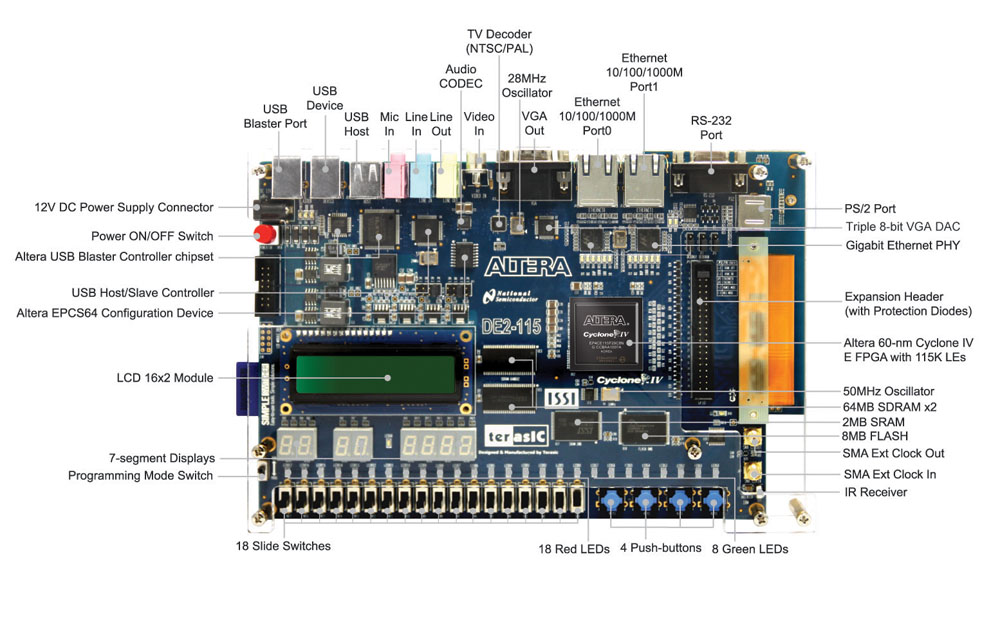
\includegraphics[width=170mm]{Lab1/figures/DE2-115.jpg}
	\caption{The DE2-115 FPGA Development Board}
	\label{fig:DE2-115}
\end{figure}

\begin{figure}[H]
	\centering
	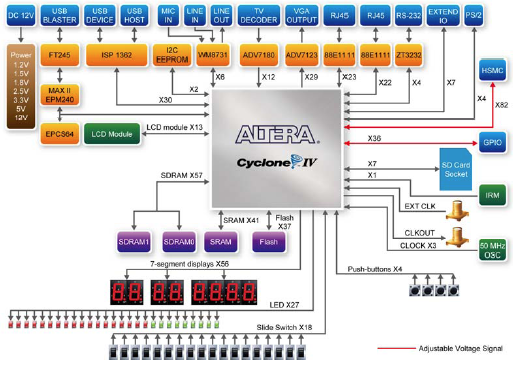
\includegraphics[width=170mm]{Lab1/figures/DE2-115Block.png}
	\caption{The DE2-115 Block Diagram}
	\label{fig:DE2Block}
\end{figure}

\subsection{Pre-Lab}

Before attempting this lab, you should complete the following:

\begin{itemize}
	\item Download and install the \emph{Quartus II 13.0 Web Edition Software} from the Altera website to your personal computer
	\item Download and read the following documents from the Sakai Resources pags;  \emph{DE2-115 User Manual}, \emph{Quartus II Introduction}
\end{itemize}
 
\subsection{Working with Quartus II}

\subsubsection{Creating a New Project}
\begin{enumerate}
	\item In order to begin working on your first FPGA project, you must open the program Altera Quartus II. To begin a new project goto  {\bf File $\rightarrow$ New Project Wizard} as shown in figure \ref{fig:step1}

	\begin{figure}[H]
		\centering
		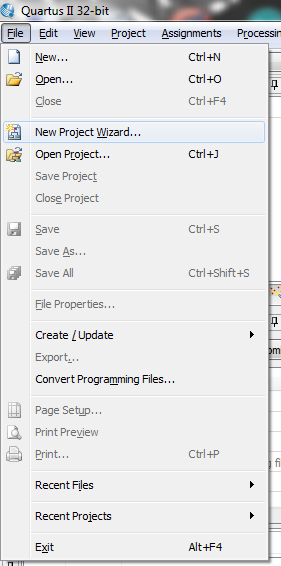
\includegraphics[width=45mm]{Lab1/figures/step1.png}
		\caption{Create a new project menu}
		\label{fig:step1}
	\end{figure}

	\item When the \emph{New Project Wizard} window opens click {\bf NEXT}

	\item Create a folder in your Z-drive called \emph{FPGA Lab}

	\item Create a folder in FPGA Lab called \emph{lab1}

	\item Set the working directory to lab1

	\item Name the project \emph{lab1}

	\item Click {\bf NEXT} to proceed

	\item Skip this step, click  {\bf NEXT} to proceed

	\item Under Device Family select \emph{Cyclone IV E}, set the package to \emph{FBGA}, pin count to \emph{780}, and speed grade to \emph{7}. In the Available devices list, look for and select \emph{EP4CE115F29C7} as shown in figure \ref{fig:step2}.
	

	\begin{figure}[H]
		\centering
		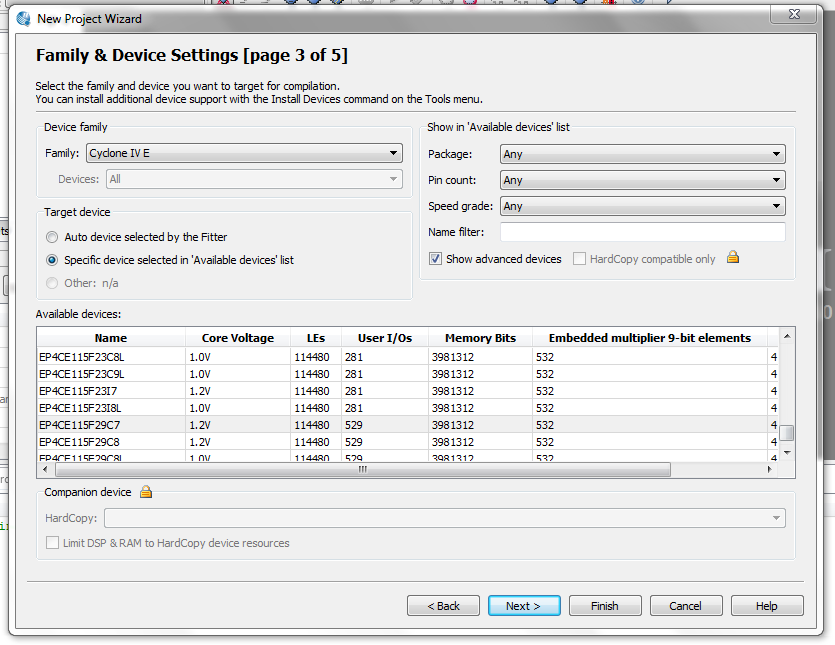
\includegraphics[width=100mm]{Lab1/figures/step2.png}
		\caption{Device selection menu}
		\label{fig:step2}
	\end{figure}

	\item Click {\bf FINISH} to begin your new project

\end{enumerate}

\subsubsection{Creating an Empty File}
\begin{enumerate}

	\item Goto {\bf File $\rightarrow$ New $\rightarrow$ VHDL File $\rightarrow$ OK } as shown in figure \ref{fig:newfile}

	\begin{figure}[H]
		\centering
		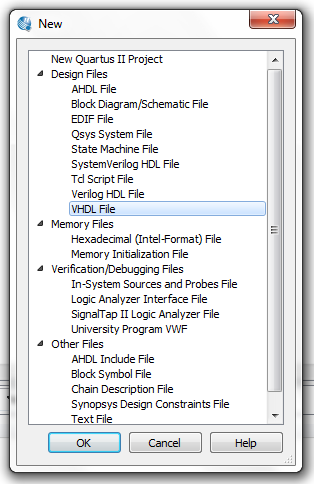
\includegraphics[width=50mm]{Lab1/figures/newfile.png}
		\caption{Create a new file menu}
		\label{fig:newfile}
	\end{figure}

	\item Save this new file by going to {\bf File $\rightarrow$ Save As $\rightarrow$ \emph{lab1.vhd} $\rightarrow$ SAVE} as shown in figure \ref{fig:saveas}

	\begin{figure}[H]
		\centering
		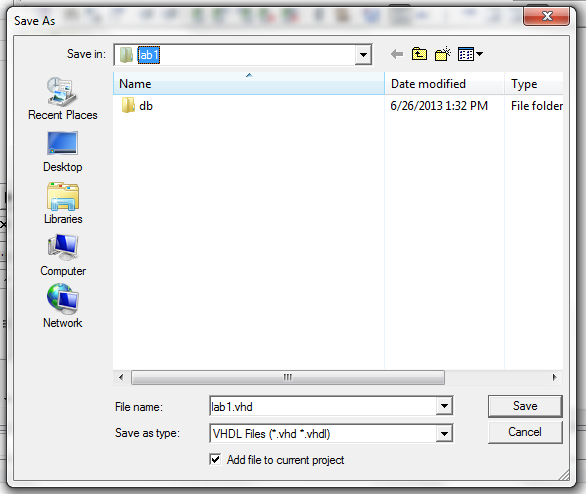
\includegraphics[width=65mm]{Lab1/figures/saveas.png}
		\caption{Save As dialog box}
		\label{fig:saveas}
	\end{figure}

\end{enumerate}

\subsubsection{Writing VHDL Code}

The following code block shows how to interact with the switches and LEDs on the DE2-115. Notice how the program begins with importing the ieee library which contains all of the basic logic primitives as established within the IEEE standard 1164. When working in industry it is common for large companies to create their own libraries as well. Every VHDL file should contain at least one entity (module) that is the same as the name of the file. An entity contains information about the structure of the module such as how many inputs/outputs (I/O) and what type of logic to expect at the I/O. Finally we define the entity in an architecture block, this section does the work on the hardware. As can be seen, this code is setting the red LEDs as defined in the array to the accompanying switches on the board. Take note on the use of comments throughout the code, comments begin with two dashes (--) and should always be used to describe what you are trying to accomplish, this way someone else who reads your code will understand it easily and your code will look more professional. 

\begin{lstlisting}
-- Import logic primitives
LIBRARY ieee;
USE ieee.std_logic_1164.all;

-- Simple module that connects the SW switches to the LEDR lights
ENTITY lab1 IS
PORT ( SW: IN STD_LOGIC_VECTOR(17 DOWNTO 0); -- Initialize switches as an input
	LEDR: OUT STD_LOGIC_VECTOR(17 DOWNTO 0)); -- Initialize red LEDs as an output
END lab1;

-- Define characteristics of the entity lab1
ARCHITECTURE Behavior OF lab1 IS
BEGIN
	LEDR <= SW; -- Assign each switch to one red LED
END Behavior;
\end{lstlisting}

\subsubsection{Setting Pin Assignments}
The Cyclone IV chip on the DE2-115 contains 780 pins. The majoprity of these pins have copper traces to the hardware the control on the development board. As a result, Altera has provided a file that contains all of the pin assignments so that you can interface directly with the pins in your VHDL code. To set the pin assignments:

 \begin{enumerate}  
 
	\item Goto {\bf Assignments $\rightarrow$  Import Assignments $\rightarrow$  Select \emph DE2-115.qsf} as shown in figure \ref{fig:importassign}.This file can be dowloaded from the Altera website
	
	\item Then click {\bf ADVANCED $\rightarrow$ check Global Assignments $\rightarrow$ Ok} as shown in figure \ref{fig:advancedimport}

\end{enumerate}

\begin{figure}[H]
	\centering
	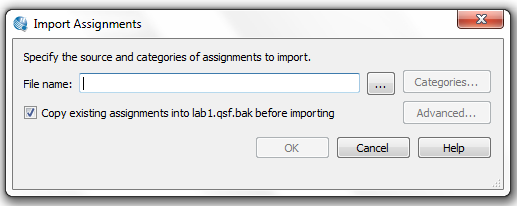
\includegraphics[width=70mm]{Lab1/figures/importassign.png}
	\caption{Import assignments dialog box}
	\label{fig:importassign}
\end{figure}

\begin{figure}[H]
	\centering
	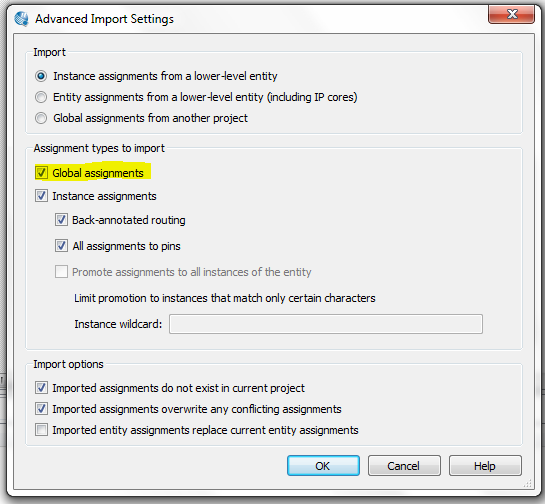
\includegraphics[width=85mm]{Lab1/figures/advancedimport.png}
	\caption{Import assignments advanced options menu}
	\label{fig:advancedimport}
\end{figure}

\subsubsection{Compiling Hardware}

\begin{enumerate}

	\item To begin compiling your hardware, {\bf Processing $\rightarrow$ Start Compilation} or you may press \emph{Ctrl + L} on your keyboard

\end{enumerate}

If the project compiles successfully, you may proceed to uploading the hardware. Otherwise if you have any errors you should debug your code. It is helpful to note that the first error should be solved first which will make it easier to solve the other errors. A succefull compilation will look like figure \ref{fig:compileresuts}.

\begin{figure}[H]
	\centering
	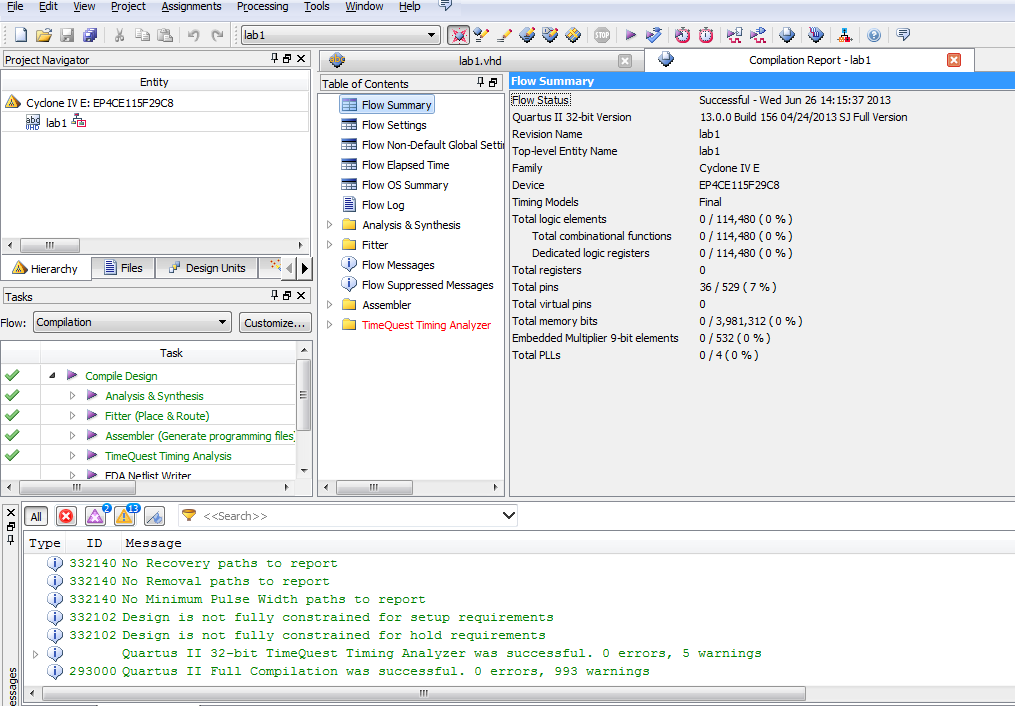
\includegraphics[width=100mm]{Lab1/figures/compileresults.png}
	\caption{Successful completion of compilation}
	\label{fig:compileresuts}
\end{figure}

\subsubsection{Testing Hardware with Waveforms}

All hardware implementations should be tested for correctness before uploading to the FPGA device. To accomplish this, please follow the tutorial titled \emph{Quartus\_II\_Simulation.pdf} listed under Sakai resources.

\subsubsection{Uploading Hardware to Device}

Once the hardware has compiled successfully, goto {\bf Tools $\rightarrow$ Programmer} to open the hardware upload options. There are two typical modes for uploading hardware and it is important to understand when to use them. This can be seen in figure \ref{fig:uploadmethod}.


\begin{figure}[H]
	\centering
	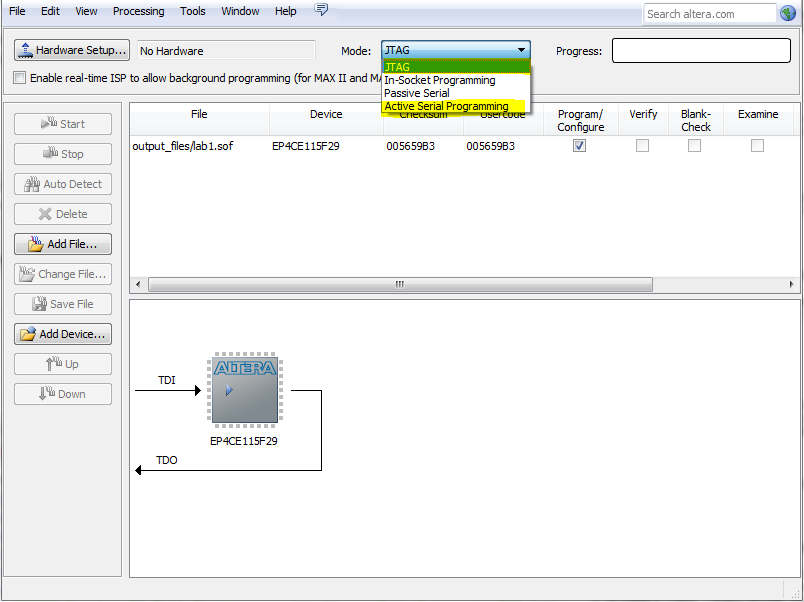
\includegraphics[width=100mm]{Lab1/figures/uploadmethod.png}
	\caption{Modes for uploading hardware to the FPGA device}
	\label{fig:uploadmethod}
\end{figure}

\begin{enumerate}

	\item JTAG or Joint Test Action Group

	\begin{itemize}
	
		\item This method loads the hardware directly to the FPGA chip
		
		\item The FPGA is unable to save its current state so if the power is turned off the programmed hardware will disappear
		
		\item To program the FPGA with this method all you need to do is connect the USB cable to the development board and ensure that under {\bf Hardware Setup} that USB-Blaster is selected. Then you must goto {\bf Add Files} and add your compiled \emph{lab1.sof} file
		
		\item Press {\bf START} to upload your hardware, in a few moments you should see your development board behaving as instructed by your code
		
	\end{itemize}

\item Active Serial

	\begin{itemize}
		\item This method loads the hardware on to the on-board configuration device. What this means is that the hardware description is saved into memory and is loaded onto the FPGA chip whenever the board is powered on. This method is more desirable because it allows the FPGA to work without being connected to the computer and only to an external power source.
		
		\item Before beginning this method you should first check that under {\bf Assignments $\rightarrow$ Device $\rightarrow$ Device and Pin Options} are configured in the same way as figure \ref{fig:activeserialconfig}, if not you must set the configuration scheme to \emph{Active Serial} and also set  the configuration device to \emph{EPCS64}. If this was not set you must recompile your hardware.

		\begin{figure}[H]
			\centering
			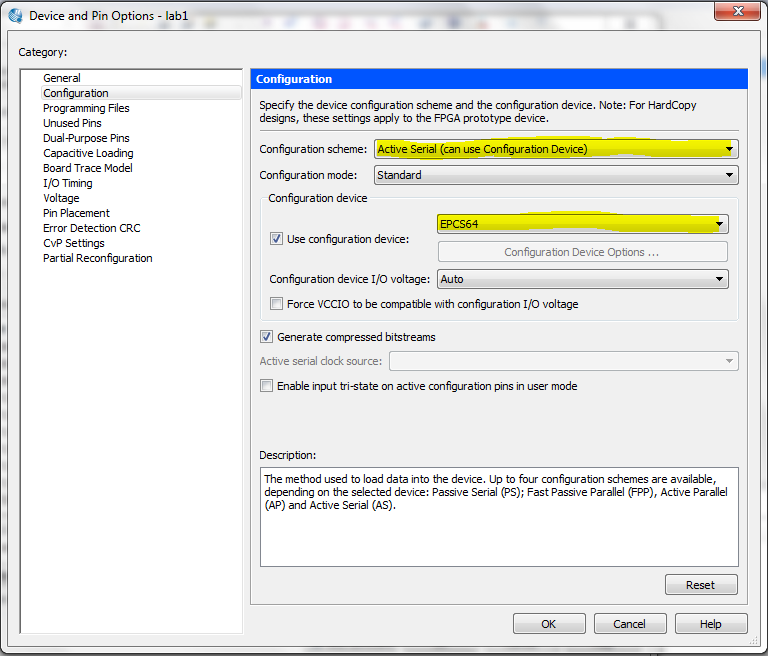
\includegraphics[width=100mm]{Lab1/figures/activeserialconfig.png}
			\caption{Active Serial Configuration Settings}	
			\label{fig:activeserialconfig}
		\end{figure}

		\item Next once again ensure that the hardware is set to \emph{USB-Blaster} and that the mode is set to \emph{Active Serial}
		
		\item Click on {\bf Add Files}, and select \emph{lab1.pof}
		
		\item Ensure that the development board is switched to \emph{PROG}
		
		\item Click {\bf START} to begin programming. This method takes slightly longer
		
		\item Switch the board back into the \emph{RUN} position and verify that your logic is behaving properly
		
	\end{itemize}

\end{enumerate}

\subsection{Activities}

\subsubsection{Implementing Logic}

Implement the hardware from the circuit in Figure \ref{fig:circuit1}. The inputs should come from SW(1) and SW(2) and the output should be shown on any of the available LEDs. Use the implemented circuit to test and create a truth table with your results and place it within a comment in the program file.

\begin{figure}[H]
	\centering
	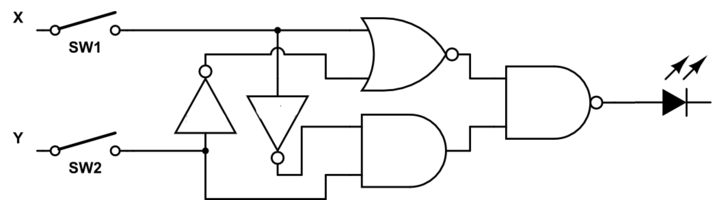
\includegraphics[width=100mm]{Lab1/figures/circuit1.png}
	\caption{Circuit for activity 1}
	\label{fig:circuit1}
\end{figure}

\subsubsection{7 Segment Display Decoder}

The 7-segment display is comprised of 7 LEDs that are arranged in such a way that allows for the creation of the numbers 0-9 and a select few characters with some clever use. Figure \ref{fig:7seg} shows the block diagram and output table. Your task is to create a 3 input, 7 output decoder that will display a number from 0-6. To accomplish this task, you should program the switches SW(0) - SW(6) to make the first 7 displays show the numbers 0-6 when its switch is turned on.

\begin{figure}[H]
	\centering
	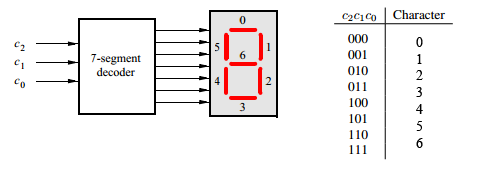
\includegraphics[width=100mm]{Lab1/figures/7seg.png}
	\caption{7 segment display and decoder}
	\label{fig:7seg}
\end{figure}

{\bf Tips:} 
\begin{itemize}
  \item The eight 7 segment displays can be accessed with the 7-bit signal vectors HEX0\ldots HEX7. For example, to output to the first display (HEX0) you can either set each bit individually (HEX0(5) <= `1';) or set the whole vector with (HEX0 <= `1111111') which would display the number 8. 
\item more to come...
\end{itemize}

\subsection{Lab Report}

Your lab report should be upload to Sakai in a zip folder that includes the following:

\begin{itemize}
	\item Commented VHDL code that clearly explains your thought process
	\item A report that 
\end{itemize}




\newpage

\section{Lab 2 - Latches, Flip-Flops, and Counters}

\subsection{Introduction}
Elementary latches and flip-flops have been used for years as a means to store temporary data either from the outputs of logic operations or by setting them to configure logic to behave in certain ways. This lab will go into the aspects of creating latches and flip-flops which will then be used to create a counter. 

\subsection{Pre-lab}
Before you begin this lab you should complete the following and upload to Sakai:

\begin{itemize}
	\item Write down the truth table for a D-latch, SR-latch and J-K flip-flop
	\item Design a block diagram for an 8-bit counter using J-K flip-flops
\end{itemize} 

\subsection{Lab Activities}

\subsubsection{Latches}
The following VHDL code implements the logic for a D-latch based off of the schematic in figure \ref{fig:dlatch}. 

\begin{lstlisting}
-- A gated D latch
LIBRARY ieee;
USE ieee.std_logic_1164.all;

ENTITY dlatch IS
	PORT (	Clk, D	: IN	STD_LOGIC;
			Q, Qbar	: OUT	STD_LOGIC);
END dlatch;

ARCHITECTURE rtl OF dlatch IS

	SIGNAL D1, D2, Qa, Qb : STD_LOGIC; -- Intermediate signals
	ATTRIBUTE keep: boolean; -- For waveform results
	ATTRIBUTE keep of D1, D2, Qa, Qb : signal is true;
	
BEGIN
	
	D1 <= NOT (D AND CLK);
	D2 <= NOT (D1 AND CLK);
	Qa <= NOT (D1 AND Qb);
	Qb <= NOT (D2 AND Qa);

	Q <= Qa;
	Qbar <=Qb;
	
END rtl;
\end{lstlisting}


\begin{figure}[H]
	\centering
	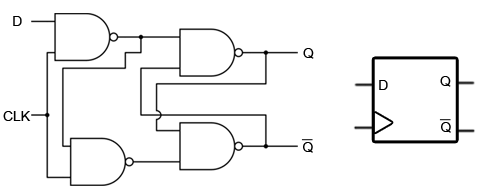
\includegraphics[width=100mm]{Lab2/figures/dlatch.png}
	\caption{D-latch circuit and block diagram}
	\label{fig:dlatch}
\end{figure}

Using this as a reference, design VHDL for an SR-latch with a clock input. Verify with waveforms that the circuit behaves the same as the truth table you created in the pre-lab.


\subsubsection{Flip-Flop}
Design VHDL code that implements the logic for a J-K flip-flop from figure \ref{fig:jkflipflop}. Verify with waveforms that the circuit behaves the same as the truth table you created in the pre-lab 

\begin{figure}[H]
	\centering
	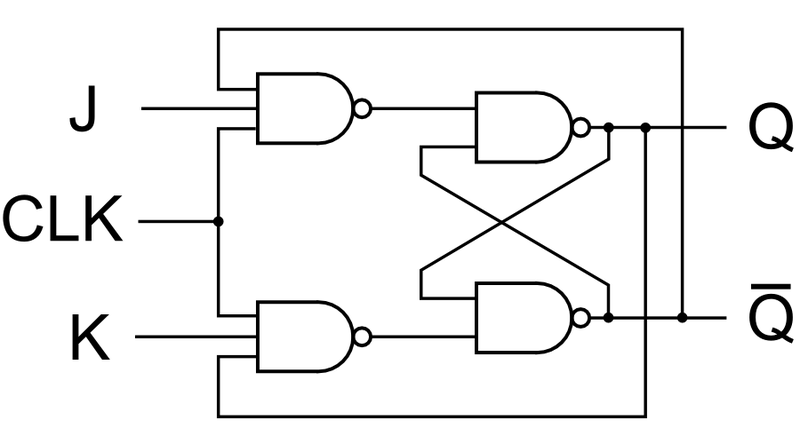
\includegraphics[width=100mm]{Lab2/figures/jkflipflop.png}
	\caption{J-K fip-flop circuit}
	\label{fig:jkflipflop}
\end{figure}

\subsubsection{Counters}
In the pre-lab, you created a block diagram for an 8-bit counter using J-K flip flops. Using the same VHDL code you created for implementing the J-K flip-flop, implement an 8-bit counter that increments when you press KEY0 on the DE2-115 development board. Link the binary output of the flip-flops to the red LEDs and then convert the binary value into hexadecimal to be shown on the 7-segment displays. \emph{Hint: you should refer to your code for the 7-segment display driver designed in the previous lab}

\subsection{Lab Report}
After completing the activities in this lab you should create a zip folder with the following and then submit it to Sakai:

\begin{itemize}
	\item Commented VHDL code
	\item VHDL test benches for all activities
	\item Waveforms for all activities
	\item A discussion on the results of compilation including longest path delay, the total number of logic elements used, and issues you encountered while performing the lab
\end{itemize}

\newpage

\section{Lab 3 - Complex Addition Systems}

\subsection{Introduction}
From your pocket calculator to inside modern CPUs adders have long been used as more than just a simple way to sum numbers together. This lab will go into the logic structure of the adder as well as provide a method for converting the simple full adder in to an \emph{arithmetic logic unit} (ALU) capable of handling 10 operations.

\subsection{Pre-lab}
Before coming to the lab, please complete the following and upload to Sakai:
\begin{itemize}
	\item A truth table for a half adder and a full adder
	\item The logic equation for a 4-bit ripple carry adder
\end{itemize}

\subsection{Lab Activities}

\subsubsection{Half Adder}
Build the circuit in Figure \ref{fig:halfadder}, create a test bench and verify that the logic is correct.

\begin{figure}[H]
	\centering
	
\includegraphics[width=60mm]{Lab3/figures/halfadder.png}
	\caption{Circuit for a 1-bit half adder}
	\label{fig:halfadder}
\end{figure}

\subsubsection{Full Adder}
The circuit in Figure \ref{fig:fulladder} implements a full 1-bit adder. Implement this circuit in VHDL, create a test bench, and verify that the logic behaves as expected. 

\begin{figure}[H]
	\centering
	
\includegraphics[width=80mm]{Lab3/figures/fulladder.png}
	\caption{Circuit for a 1-bit full adder}
	\label{fig:fulladder}
\end{figure}

Now that you have a working 1-bit full adder, implement a 4-bit ripple carry adder that sums the binary numbers "0110" and "0101." A block diagram for the 4-bit ripple carry adder is shown in Figure \ref{fig:fourbitripple}. Verify your results by creating a test bench and simulating the circuit.

\begin{figure}[H]
	\centering
	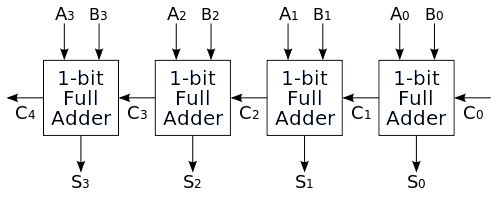
\includegraphics[width=100mm]{Lab3/figures/fourbitripple.png}
	\caption{4-bit ripple carry adder block diagram}
	\label{fig:fourbitripple}
\end{figure}

\subsubsection{Full Adder Based ALU}
The block diagram in Figure \ref{fig:fulladderalu} is an example of how the regular 1-bit full adder can be manipulated to implement additional functionality. For this activity, you must build VHDL code that implements a 4-bit complex adder ALU, the list of instructions can be found in Table \ref{tab:adderaluop}.

\begin{figure}[H]
	\centering
	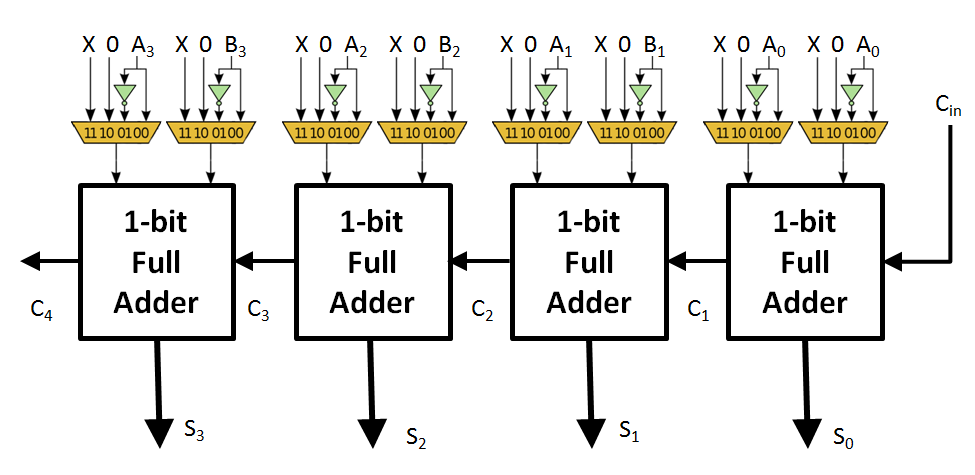
\includegraphics[width=150mm]{Lab3/figures/fulladderalu.png}
	\caption{Block diagram for a 4-bit ripple carry adder ALU with 10 operations}
	\label{fig:fulladderalu}
\end{figure}

After writing and testing your VHDL code, upload it on the DE2-115 FPGA Development board. Connect the inputs {\bf A0-A3} to SW0 - SW3 and the inputs {\bf B0-B3} to SW4 - SW7. Also connect {\bf D$_0$} to SW8 and {\bf D$_1$} to SW9. Display inputs {\bf A} and {\bf B} in hexadecimal on HEX0 and HEX2, respectively and the output {\bf S} on HEX4. If the result over-flows display {\bf C$_4$} on LEDG0. If the result is negative turn on LEDR0 and if it is zero turn on LEDR1. Test and verify all ten operations and take a picture of each result (make a table that includes the values for {\bf A}, {\bf B}, {\bf S}, {\bf C$_4$}, {\bf Neg}, and {\bf Zero}.

\begin{table}[H]
	\centering
	\caption{List of opperations for the adder based ALU}
	\begin{tabular}{ | c | c | c | c | }
		\hline                        
 		\bf A$_i$ & \bf B$_i$ & \bf D$_0$ D$_1$ & \bf Result \\ \hline
 		Set to 0 & Set to 0 & 00 & 0 \\ \hline
 		Set to 0 &  Set to 0 &10 & 1 \\ \hline
 		A &  Set to 0 & 00 & A \\ \hline
 		Set to 0& B  & 00  & B  \\ \hline
 		A & Set to 0 & 10 & A $+$ 1 \\ \hline
 		Set to 0 & B & 10 & B $+$ 1 \\ \hline
 		A & B & 00 & A $+$ B \\ \hline
 		A & B & 10 & A $-$ B \\ \hline
 		Set to invert & Set to 0 & 01 & $\overline{A}$ \\ \hline
 		Set to invert & Set to 0 & 11 & $-$A \\ 
 		\hline
	\end{tabular}
	\label{tab:adderaluop}
\end{table}

When you finsih building the VHDL upload your code to the FPGA board. Test and verify all ten operations and take a picture of each result (make a table with that includes the values for {\bf A, B, S, C$_4$, Neg, and Zero}.

\subsection{Lab Report}
After completing the activities in this lab you should create a zip folder with the following and then submit it to Sakai:

\begin{itemize}
	\item Commented VHDL code.
	\item VHDL test benches for the half adder and full adder activities.
	\item Waveforms for the half adder and full adder activities.
	\item Pictures of the results from the ALU activity.
	\item A discussion on the results of compilation including longest path delay, the total number of logic elements used, and issues you encountered while performing the lab.
\end{itemize}



\newpage

\section{Lab 4 - Finite-State Machines}

\subsection{Introduction}
A \emph{finite-state machine} (FSM) is a model for sequential logic that consists of a set of states (including an initial or reset state) a set of inputs/outputs and a transition function that shows the transition from one state to other states. The state the FSM is in at any given time is called the {\it current} state. The FSM can change from one state to another when initiated by a triggering event or condition (input); this is called a transition. This lab will examine a simple FSM to give the general idea of how they work, and build upon it to create a system modeled off of a real world example, a vending machine.

\subsection{Pre-lab}

Before coming to the lab, please complete the following activity and upload the results to Sakai.
\begin{itemize}
	\item By examining the code in Listing \ref{code:fsm} write out its state machine transition graph.
\end{itemize}


\subsection{Lab Activities}

\subsubsection{FSM}

Given the state machine transition graph in Figure \ref{fig:fsm}, design VHDL code for the state transitions of this diagram. Note that in the state transition graph, we show the transition behavior as input/output where the input is denoted as D$_1$D$_0$ and the output is denoted as  Z$_1$Z$_0$. For example 00/01 means D$_1$D$_0$ = 00 and causes  Z$_1$Z$_0$ = 01. Assume that state A is the reset state for this machine.

\begin{figure}[H]
	\centering
	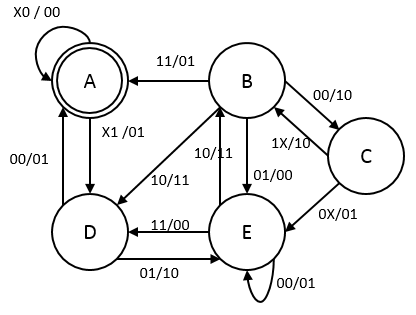
\includegraphics[width=100mm]{Lab4/figures/fsm.png}
	\caption{State machine transition graph}
	\label{fig:fsm}
\end{figure}

The code below shows a simple example of a FSM. You can build upon this code in completing this lab. 

\begin{lstlisting}[caption=Sample code for a Finite State Machine, label=code:fsm]
-- User-Encoded State Machine
library ieee;
use ieee.std_logic_1164.all;

entity state_machine is
	port(clk	 	 : in std_logic;
		reset	  : in std_logic;
		input	  : in std_logic;
		output	  : out std_logic);
	
end entity;

architecture rtl of state_machine is
	-- Build an enumerated type for the state machine
	type count_state is (A, B, C, D);
	
	-- Registers to hold the current state and the next state
	signal present_state, next_state	   : count_state;
	
	-- Attribute to declare a specific encoding for the states
	attribute syn_encoding				  : string;
	attribute syn_encoding of count_state : type is "11 01 10 00";
	
begin
	-- Move to the next state
	process(clk, reset)
	begin
		if reset = '1' then
			present_state <= A;
		elsif (rising_edge(clk)) then
			present_state <= next_state;
		end if;
	end process;

	-- Determine what the next state will be, and set the output bits
	process (present_state, input)
	begin
		case present_state is
			when A =>
				if (input = '0') then
					next_state <= B;
					output <= '0';
				else
					next_state <= D;
					output <= '0';
				end if;
			when B =>
				if (input = '0') then
					next_state <= C;
					output <= '1';
				else
					next_state <= A;
					output <= '0';
				end if;
			when C =>
				if (input = '0') then
					next_state <= D;
					output <= '0';
				else
					next_state <= B;
					output <= '1';
				end if;
			when D =>
				if (input = '0') then
					next_state <= A;
					output <= '0';
				else
					next_state <= C;
					output <= '1';
				end if;
		end case;
	end process;
	
end rtl;
\end{lstlisting}

\subsubsection{Vending Machine}

Design a custom finite-state machine to control a vending machine to dispense products. The design has the following specifications:

\begin{enumerate} 

	\item The state machine should have three states:

	\begin{itemize}
		\item \emph{IDLE}: This is the default (reset) state for the machine. The machine should stay in this state until at least one product is selected. Being that this is the reset state, you should initialize the signals QUARTERS, COST, and DISPENSE\_READY to zero. Make sure that LEDR0 to LEDR17 along with LEDG1 to LED8 are set to off. While in this state, you should display a dash across all HEX displays. 

		\item \emph{PRODUCT\_SELECT}: The state machine will move into this state if product(s) are selected through use of the switches (SW0 - SW15) on the FPGA board. Display the total cost in number of quarters needed of all products selected on HEX5 - HEX4 in hexadecimal.  KEY3 and KEY2 should increment QUARTERS by a dollar and quarter respectively when pressed. Display the value of QUARTERS on HEX1 - HEX0. When the correct number of quarters have been inserted, the signal DISPENSE\_READY should go HIGH (which should be shown on LEDG8) and the state should transition to DISPENSE. A list of available products and their cost can be found in Table \ref{tab:costlist}.

		\item \emph{DISPENSE}: Once the proper amount of quarters have been deposited, the item should be dispensed from the machine. To show that the item(s) have been dispensed, turn on LEDR0-LEDR17 and set the next state to idle.

	\end{itemize}
	
	\item KEY0 will act as a CLOCK input and KEY1 will act as a coin return or reset. The states should transition on the rising edge. This means that you should select a product and then send a CLOCK pulse to calculate the cost of the item(s) selected. Then add quarters into the machine and send another CLOCK pulse when there is the right amount of quarters. If there is not enough quarters inserted, the state should not change. Once the item(s) are dispensed, send another CLOCK pulse to return to IDLE.

	\item The current state; \emph{IDLE}, \emph{PRODUCT\_SELECT}, and \emph{DISPENSE} should be displayed by turning on LEDG0 - LEDG2 respectively.
	
	\item Both signals QUARTERS and COST should be of the type INTEGER with a range of 0 to 40. You will need to include the package \emph{ieee.numeric\_std.all}.

\end{enumerate}

\begin{table}[H]
	\centering
	\caption{List of vending machine items, cost, and switch correspondence}
	\begin{tabular}{ | c | c | c | }
		\hline                        
 		\bf Product & \bf Cost & \bf Switch\\ \hline
 		SODA\_CAN[0:3] & \$1.00 & SW12 - SW15 \\ \hline
		CHIPS[0:3] & \$0.75 & SW8 - SW11 \\ \hline
		CHOCOLATE[0:3] & \$0.50 & SW4 - SW7 \\ \hline
		BUBBLE\_GUM[0:3] & \$0.25 & SW0 - SW3 \\
 		\hline
	\end{tabular}
	\label{tab:costlist}
\end{table}


\subsection{Lab Report}

After completing the activities in this lab you should create a zip folder with the following and then submit it to Sakai:

\begin{itemize}
	\item Commented VHDL code.
	\item Waveform for the FSM activity.
	\item Pictures of the results from the vending machine activity.
	\item A discussion on the results of compilation including longest path delay, the total number of logic elements used, and issues you encountered while performing the lab.
\end{itemize}




\newpage

\section{Lab 5 - A Simple Computer}

\subsection{Introduction}
16bit simple processor

\subsection{Lab Activities}

\subsubsection{Design an ALU}
Add, Sub, Mult, Shift, XOR, AND, NAND,

\subsubsection{Design a RAM}
512 bit memory

\subsubsection{Design the Program Counter}
simple counter

\subsubsection{Create a VGA Driver}
Display the output onto the screen

\newpage

\section{Final Project}

\subsection{Introduction}
For the remainder of this course you will be required to work on and complete a project that 
\subsection{Requirements}

\subsection{Project Ideas}

\subsection{Deliverables}



\end{document}